\chapter{L'écoute}

\section{Ecouter ou entendre : une différence}

La définition du verbe ``entendre'' et du verbe ``écouter'' 
\autocite[pp. 361--385]{hachette:dictionnaire} nous paraît opportune
en raison de la confusion courante des deux termes :
\begin{description}
\item[Entendre] c'est  percevoir des sons, saisir par l'ouïe.
\item[Ecouter] a trois sens: 
\begin{enumerate}
	\item prêter l'oreille à; s'appliquer à entendre;
	\item prêter attention à l'avis de quelqu'un, suivre un avis;
	\item \emph{fig} suivre une impulsion,	une inspiration.
\end{enumerate}
\end{description}



\emph{Entendre} est une attitude passive par rapport au monde sonore
qui nous entoure. Nous recevons les sons sans les interpréter et cela
ne demande aucun effort. C'est une action involontaire et non
sélective. 

Selon Bernard Auriol\autocite[p. 2, ch	. 1]{auriol:cle}, \textit{entendre} 
\begin{quote}
	<<\,suppose un son (physique), une oreille
	pour le capter, un système nerveux pour le recevoir.\,>>
\end{quote} 
Tandis qu'\textit{écouter}
\begin{quote}
	<<\,est un
	processus actif supposant préférences et répulsions pour tel son ou
	telle séquence sonore.\,>>
\end{quote}


Entendre et écouter sont «\,deux
fonctions essentiellement distinctes bien qu'évoluant apparemment sur
des terrains identiques\,>>
% ancien texte {\textbf{site internet: http: auriol.free.fr} Extrait de l'entretien réalisé par
%	Bernard Auriol avec Alfred Tomatis, 1973.}.
[\dots] avec «\,l'élément conscient, facteur essentiel sur lequel repose toute la
différence entre ces deux activités\,».\autocite[Voir p. ?]{tomatis_oreille_1991}
\pdfmargincomment{Pages des 2 citations?}
\begin{quote}
	
	<<[\ldots] Entendre n'implique pas pour autant la pré\-sen\-ce d'un champ
	conscient. \emph{Entendre, c'est en quelque sorte subir
		un son} ou un message qui nous est adressé. \emph{Ecouter, c'est désirer appréhender ce son} ou ce message [\ldots]>>
	\autocite{tomatis:education}.	
\end{quote}



Ainsi, comme nous l'avons mentionné juste avant dans l'introduction%
\footnote{Voir point \ref{jeSuisLaMusique:viret}, p. \pageref{jeSuisLaMusique:viret}.}
\enquote{\emph{Je suis la musique que je fais ou écoute}}\autocite{viret:b}, \textbf{écouter} implique 
une conscience pour s'actualiser dans le sujet. Elle est une opération 
qui suppose une participation active dans le choix du message
ou dans la sélection d'une voix. Elle  implique la volonté,
\pdfmargincomment[color=green]{Bien!}
permet une forme de décodage: il s'agit d'une capacité. Dans un milieu sonore important,
 bruyant, comme un café, lorsque nous lisons attentivement, nous faisons abstraction
des bruits environnants; en soi, nous les entendons parfaitement mais nous n'y
prêtons pas attention. Nous parvenons à couper les sons parasites, à nous en abstraire pour
nous concentrer uniquement sur les plus  pertinents, en l'occurrence ici ceux de notre lecture intérieure.
 La racine du mot `écouter' a des origines sanskrites et signifie \emph{partager}; nous remarquons alors à juste titre que nous écoutons le plus souvent en face de quelqu'un dans le but de dialoguer, d'échanger. Le même phénomène se réalise avec un livre qui transmet et partage des connaissances. L'écoute permet donc la communication, sous-entend le plus souvent la présence d'un être en vis-à-vis et nécessite de la  concentration. Il faut cette volonté inclue dans celle-ci  pour comprendre et rentrer par exemple en contact avec la voix de  l'écrivain qui chante dans le texte avec celle, intérieure,  du lecteur.
 
 
 \textbf{Ecouter} se base certes sur une stimulation prenant sa source à 
l'extérieur mais \textbf{devant être intérieurement et  intentionnellement
	recherchée}.




Nous pouvons aussi différencier les différents types d'écoute. D'après Edith Lecourt \autocite[ch. 10 <<\,De l'écoute verbale à l'écoute musicale\,>>, p. 182.]{lecourt:decouvrir}
 on en distingue plusieurs : l'écoute verbale, musicale, plurivocale et multiple.
 L'analyse musicale qui permet la différenciation d'une voix d'un ensemble polyphonique est appelée \emph{plurivocale}. Celle qui est multiple n'est pas analytique  mais 
 \begin{quote}
 	 [\ldots] \textit{ouvre une disponibilité, met en suspens les grilles verbale et musicale} [\ldots] \emph{pour parcourir le vécu sonoro-affectif}\autocite[p. 183]{lecourt:decouvrir}.
 \end{quote}
 Employée en musicothérapie, Edith Lecourt la nomme la technique de la  \emph{communication sonore} qui peut apporter 
 <<\,des ouvertures sur l'analyse des niveaux plus archaïques de l'organisation mentale.\,>>\autocite[p. 154]{lecourt:decouvrir}	
 Par l'expérience musicale en groupe, il peut y avoir un moment particulier, de ``grâce"  nommé ``le concept d'illusion groupale", l'illusion d'une unité absolue, comme un seul corps\autocite{anzieu:groupal} dont parle Didier Anzieu.

 Nous aborderons plus loin ce lien au chapitre \ref{musicothEtpsycho} intitulé <<\,La musicothérapie et la psychothérapie\,>>.
 
 
Puisque \emph{écouter} implique la notion de \emph{son} et d'\emph{oreille}, nous allons dans un premier temps approfondir  la définition du son et ses caractéristiques physiques puis dans un deuxième temps aborder l'anatomie de l'oreille.

\section{Le son}

Le son possède plusieurs caractéristiques physiques. Il peut être
défini très précisément par un ensemble d'unités physiques chiffrées
: les décibels  et les hertz. 

\subsection{Unités de mesure}

Un décibel\autocite[In Wikipedia]{noauthor_decibel_2018} (\SI{}{\decibel} ) est l'unité de mesure de l'intensité du son.
 Un décibel est égal à $1/10$ de bel (\SI{}{\bel}):
	$$\SI{1}{\decibel} = \SI{1/10}{\bel} $$
	 Une augmentation de l'intensité égale à \SI{1}{\bel}
équivaut à peu près à un doublement de l'intensité sonore.
	 
	
Un hertz (\si{\hertz}) est une unité de fréquence\footnote{La fréquence est le nombre de vibrations par unité de temps dans un
		phénomène périodique.}. Équivalent à $\SI{1}{\second - 1} $. Fréquence d'un phénomène périodique
	dont la période est une seconde. \pdfmargincomment{Je laisserais tomber les multiples etc.} Ses multiples sont, entre autres,
	le kilohertz (\si{\kilo\hertz}), le mégahertz (\si{\mega\hertz}) et le gigahertz (\si{\giga\hertz}). Cette
	unité vient du savant allemand Heinrich Hertz, pionnier de la radioélectricité.

\subsection{Deux définitions du son}

Le son peut être défini de deux manières.

\subsubsection{Définition objective}

C'est le phénomène phy\-si\-que
d'origine mécanique consistant en une variation de pression (très
faible), de vitesse vibratoire ou de densité du fluide, qui se propage
en modifiant progressivement l'état de chaque élément du milieu considéré,
donnant ainsi naissance à une onde acoustique (la propagation des
ronds dans l'eau suite à un ébranlement de la surface donne une bonne
représentation de ce phénomène). 

\subsubsection{Définition subjective}	

	Il s'agit de la sensation procurée
	par cette onde, qui est reçue par l'oreille, puis transmise au cerveau
	et déchiffrée par celui-ci.\footnote{www.futura-sciences.com \pdfmargincomment{Page stp?}} 
	\index{http://www.futura-sciences.com/sante/dossiers/medecine-bruit-effets-sante-259/page/3}

De plus, il y a de nombreux paramètres à prendre en compte, comme par
exemple l'impression de force sonore : la sensibilité de l'oreille
est une variable de la fréquence. Il faut 1000 fois moins de pression
acoustique pour avoir une sensation auditive à \SI{4000}{\hertz} qu'à \SI{50}{\hertz}.
Notre oreille n'a donc pas la même sensibilité pour toutes
les fréquences audibles. Il en est de même pour la sensation auditive
des basses fréquences et pour la dynamique. 

\subsubsection{Ecoute objective ou subjective?}

Nous avons tous,
selon les manuels d'anatomie, la même
oreille, du moins nous pouvons reconnaître une analogie de structure. Nous devrions donc entendre et écouter la même chose
lors d'une même information diffusée tout comme le fait un enregistreur avec un micro. Pourtant il n'y a pas d'écoute \emph{passive}. Chacun n'entend pas de la même manière les mêmes
informations. En somme, tout un chacun entend ce qu'il veut bien
entendre, selon sa propre psyché. 

 \emph{Vouloir voir, c'est viser.}  Vouloir entendre dans le but d'écouter est comparable  à
la visée de l'\oe il lorsque l'on veut collecter une information. L'\oe il regarde avec la rétine et  vise, sous l'ordre du cerveau, avec la macula. Dans la même idée, par l'écoute, nous avons l'oreille et la cochlée (partie interne de l'oreille) qui permet l'analyse des sons. A nouveau, il faut une commande du cerveau.
En définitive, \textbf{ l'audition est la capacité perceptive du système auditif et l'écoute, c'est ce qu'on en fait.}

\subsection{Le cerveau}

Nous nous apercevons du rôle important que peut jouer notre cerveau à cet égard et de son énorme complexité.
Les recherches scientifiques sont très abondantes à ce sujet et les publications n'en finissent pas de paraître.
Nous relèverons pourtant ceci: 

Ce que Descartes nous avait inculqué trois siècles auparavant avec le "Je pense donc je suis" a été bouleversé par Antonio Damasio \footnote {{L'erreur de Descartes}, Antonio Damasio, Ed.Odile Jacobs, 1997} 
avec sa découverte de l'intelligence émotionnelle, indispensable au fonctionnement du cerveau, l'intelligence cognitive ne suffisant pas. 
\footnote{"\{Notre cerveau n'a pas fini de nous étonner", Entretien avec Jean-Michel Oughourlian, pp.118--119, Ed. Albin Michel, Le Livre de Poche 2012 }}
Et nous avons  également le troisième cerveau, le mimétique avec les neurones miroirs que Giacomo Rizzolatti avait découvert en 1990.
 
La découverte de cette intelligence  émotionnelle est donc essentielle  pour la musicothérapie puisqu'elle reconnaît implicitement le rôle important de la musique sur l'émotion.  L'IRM fonctionnelle 
(Imagerie par Résonance Magnétique)  permet d'avoir une vision globale de 
l'activité du cerveau lorsque celui-ci est soumis à une stimulation 
sensorielle. Toutes les expériences accumulées depuis des siècles en musicothérapie,
tous les résultats cliniques trouvent aujourd'hui leur confirmation par les remarquables
avancées des sciences humaines. 
Emmanuel Bigand,  chercheur, professeur de psychologie cognitive à l'Université 
de Bourgogne, nous rend attentif à  l'aspect paradoxal de la musique, 
sa structure sans fonction biologique précise mais qui fait réagir 
fortement l'être humain en activant  le cerveau autant que la nourriture 
ou la drogue.\autocite[Voir ch. 3 p. 35, "Vous avez l'oreille musicale"]{bigand:cerveau}
Grâce aux travaux d'Isabelle Peretz%
\autocite[<<\,Les agnosies auditives\,>>, pp. 205--216]{seron.baron.ea:neuropsychologie}
ainsi qu'au chercheur français, Hervé Platel,% 
\autocite[pp. 223--224]{platel_neuropsychology_2002}
on sait actuellement que \enquote{le cerveau traite distinctement les aspects perceptifs et émotionnels de la musique},
que \enquote{les circuits neuronaux qui concernent la mémoire musicale à long terme 
sont distincts des processus neurofonctionnels sollicités pour la mémoire verbale.}.
% OGA: référence de cette dernière citation stp
% OGA: vérifie stp la référence automatique. Tu avais mis chap. 4 etc.
% mais cela a changé au fil des modifications. Je ne peux pas me
% référer à une numéro de note automatiquement: page, section.
Nous verrons encore plus loin\footnote{Chap. 4, p. 34, note 24. Voir \ref{bascule}, p. \pageref{bascule}.} 
le lien important entre la difficulté à percevoir certains sons et l'existence 
de troubles émotionnels, recherche du CNRS, \pdfmargincomment{Prénoms en entier stp}
menée par S. Aubert-Khalfa, J . P . Granier, E. Reynaud, M. El Koury, O. Blin.


est difficile de clore ce sujet passionnant et nous aimerions tout de même rajouter ceci à propos de l'écoute et du cerveau : quoique
  le domaine de recherche sur l'autisme soit encore en pleine investigation et que rien n'ait été encore défini, il semblerait que la capacité d'entendre des patients autistes soit excessive, qu'il s'agit d'une hypersensibilité aux sons devenant douloureuse quand  le flux des informations est trop important et que le tri ne peut pas se faire. Le cerveau entend mais ne veut pas ou ne peut plus  écouter, pour en réalité, se protéger.

 L'autisme reste difficile à élucider. Selon Brigitte Harisson,  
 les dernières recherches sur le TSA (trouble du spectre autistique) affirmeraient que leur cerveau soit différemment connecté et qu'il ne s'agit pas d'une déficience intellectuelle ni d'une maladie mais d'un trouble neuro-développemental, un trouble
  d'intégration sensorielle.\autocite[Cet ouvrage propose une description unique du TSA (trouble du spectre de l'autisme). Voir pp. 22--23]{harrisson.st-charles:lautisme}






\section{L'oreille}


\begin{quotation}
	\char`\"{}\textbf{C'est le son qui a fabriqué l'oreille et si tu veux connaître
		le son, apprends d'abord à étudier l\textquoteright oreille\char`\"{}.}
	Hermès Trimégiste \pdfmargincomment{Tu as la référence?}
\end{quotation}

\subsection{L'anatomie de l'oreille}
\begin{figure}
	\centering
	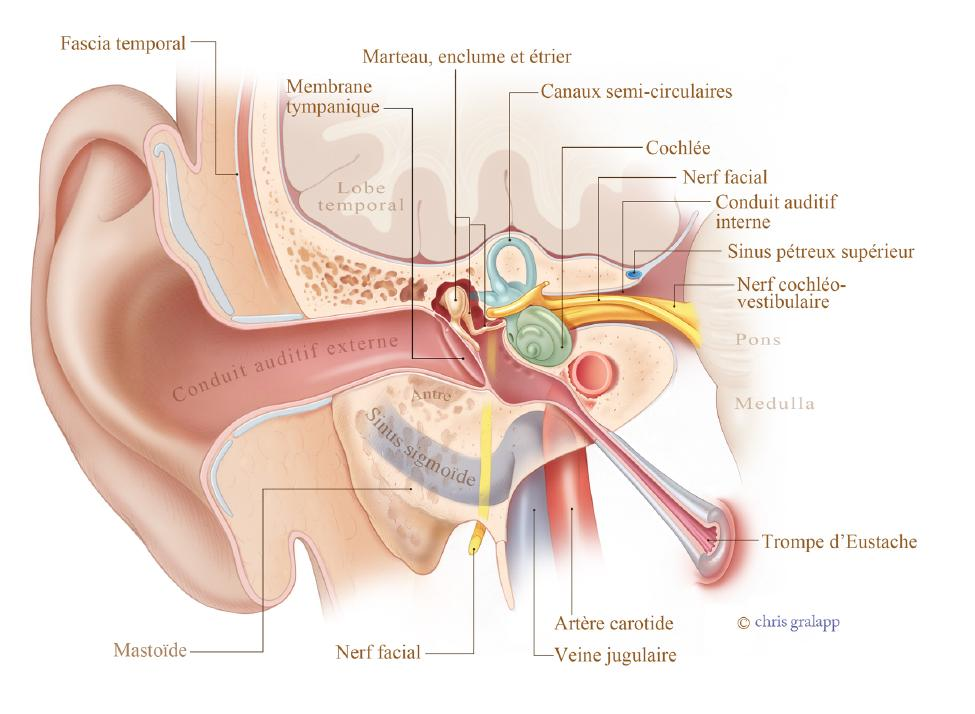
\includegraphics[width=0.7\linewidth]{images/20160624Berufsfeldgruppen.jpg}
	\caption[Anatomie oreille]{Anatomie de l'oreille}
	\label{fig:-20160624berufsfeldgruppen}
\end{figure}

L'oreille\autocite[ch. 8 pp. 319--321]{marieb:biologie} 
se situe à l'intérieur de l'un des os du crâne, le temporal, et plus précisément la pyramide pétreuse ou rocher. Elle se compose de trois parties : externe, moyenne, interne.

\subsubsection{L'oreille externe}

L'oreille externe\autocite[ch. 8, pp. 319--321.]{marieb:biologie}
est formée du pavillon et du méat acoustique externe
	(canal auditif). Les ondes sonores entrent dans le méat et percutent
	une membrane de \SI{60}{\milli\metre\squared}, appelée tympan, et la font vibrer. Cette membrane
	sépare l'oreille externe de l'oreille moyenne. 
	Selon Alfred Tomatis, médecin audio-psycho-phonologue dont nous reparlerons plus loin,
	% au chapitre 3.3/ 4, 
	elle joue un rôle de filtre des graves et d'amplificateur des aigus.




\subsubsection{L'oreille moyenne}

L'oreille moyenne se trouve dans l'os temporal constituée de petites
cavités dont une, centrale, qui est la caisse du tympan. Sa limite
médiale est une paroi osseuse percée de deux orifices, la fenêtre
du vestibule et la fenêtre de la cochlée. La trompe auditive ou d'Eustache
est un conduit oblique qui relie l'oreille moyenne à la gorge et sert
à équilibrer la pression de l'air entre l'oreille moyenne et l'extérieur.
Les trois osselets de l'ouïe sont : le marteau, l'enclume et l'étrier
(les plus petits os du corps). Ils transmettent les vibrations du
tympan aux liquides de l'oreille interne. Le marteau et l'étrier se
trouve dans l'os temporal constituée de petites cavités dont une,
centrale, qui est la caisse du tympan. 
% OGA: répétition ici, c'est pourquoi j'ai commenté
%Les trois osselets de l'ouïe
%sont : le marteau, l'enclume et l'étrier (les plus petits os du corps);
Le marteau et l'étrier sont commandés chacun par un muscle. D'après
Tomatis, son rôle est double : protéger l'oreille interne des sons
trop forts et celui de cibler les sons à écouter.

\subsubsection{L'oreille interne et le labyrinthe osseux}

\begin{figure}
	\centering
	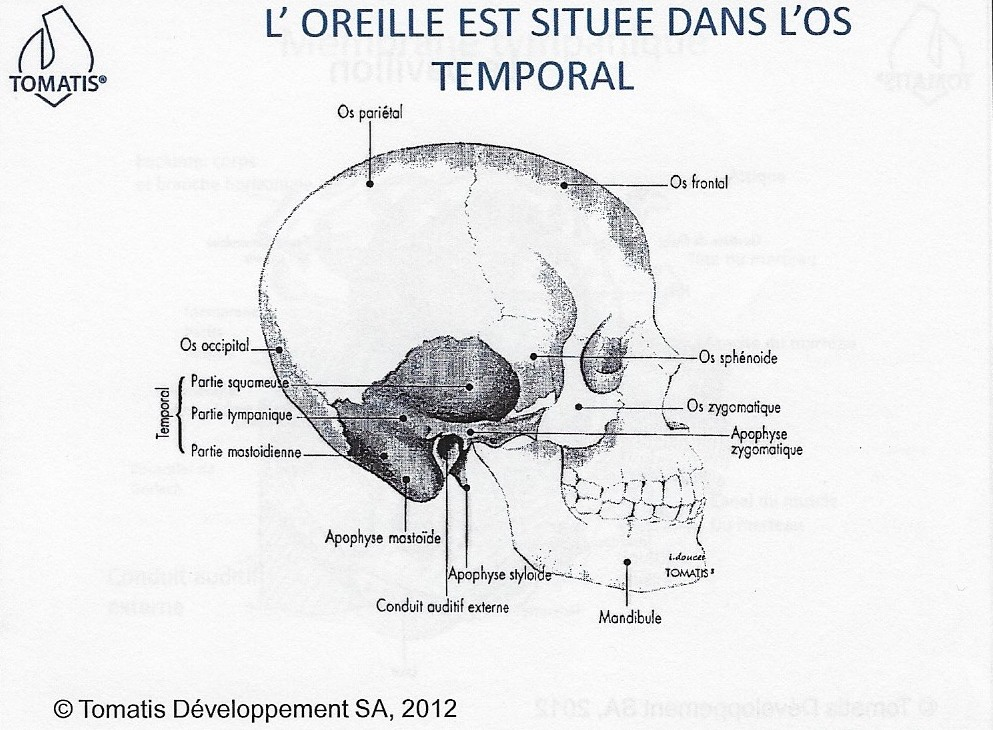
\includegraphics[width=0.7\linewidth]{images/Loreilleostemporal_crane.jpg}
	\caption[L'os temporal]{L'os temporal}
	\label{fig:loreilleostemporal18}
\end{figure}

L'oreille interne est l'organe de l'audition. Il
est constitué d'une coque osseuse d'une très grande densité (la plus
importante du corps), contenant un corps membraneux qui en épouse
la forme. 
L'oreille interne est une enfilade de cavités osseuses portant 
le nom de \emph{labyrinthe osseux}. Il comprend trois subdivisions : 
\begin{enumerate}
	\item la cochlée;
	\item le vestibule du labyrinthe;
	\item  les canaux semi-circulaires.
\end{enumerate}

Le labyrinthe
osseux est rempli de périlymphe, un liquide. Et dans ce périlymphe
flotte le labyrinthe membraneux qui contient lui-même un liquide
plus épais appelé endolymphe. Ils jouent leur rôle dans l'équilibre
statique et dynamique. Le vestibule et les canaux semi-circulaires
sont les organes de l'équilibration; la cochlée ou
limaçon est l'organe de l'audition. 

\subsubsection{Le canal auditif}
\pdfmargincomment[color=yellow]{répétition avec oreille externe}
Les ondes sonores entrent dans le méat et percutent
une membrane de \SI{60}{\milli\metre\squared} appelée \emph{tympan}, et la font vibrer. Cette membrane
sépare l'oreille externe de l'oreille moyenne. Selon Tomatis, elle
joue un rôle de filtre des graves et d'amplificateur des aigus.



\section{La physiologie de l'audition}

Le \pdfcomment[voffset=5pt]{sous-section? Sinon une phrase} chemin du son dans 
l'oreille\autocite[chap. 8, pp. 322--324]{marieb:biologie} jusqu'au cerveau.

Chaque son parvenant à l'oreille entre dans le pavillon et se propage
dans le conduit auditif. Les vibrations de l'onde sonore mettent en
mouvement le tympan lié aux trois petits os (marteau, enclume, étrier).
La transformation (et l'amplification) des vibrations
aériennes en vibrations solidiennes se fait par l'intermédiaire
des osselets : les vibrations du tympan entraînent successivement
celles du bloc marteau-enclume puis celle de l'étrier,
qui les transmet à l'oreille interne via la fenêtre
ovale.

Le rapport de levier effectif entre le marteau et l'enclume
(de l'ordre de 20), d'une part, et le
rapport de surfaces entre le tympan et la platine de l'étrier
(\SI{30}{\milli\metre\squared}) d\textquoteright autre part font du système tympano-ossiculaire
un véritable amplificateur permettant à l\textquoteright énergie sonore
d\textquoteright être transmise presque intégralement à l\textquoteright oreille
interne.

A partir de 80 dB, un réflexe protecteur (stapédien) est mis en place
afin de réduire la transmission des pressions vers l\textquoteright oreille
interne, par l\textquoteright intermédiaire des osselets et des muscles
qui rattachent le marteau et l\textquoteright étrier aux parois de
la caisse du tympan. Il s'agit ainsi d' un procédé mécanique qui amplifient
les vibrations atteignant la cochlée. 
\begin{quotation}
	La cochlée à son tour ``va transformer ces vibrations en impulsions
	nerveuses véhiculées par le nerf auditif.'' (\dots) Les cellules ciliées
	tapies dans la membrane cochléaire ``transforment ces vibrations
	en messages électriques, circulant dans le nerf auditif. (\dots) Et
	ces informations vont ``se diriger vers le cortex cérébral, via plusieurs
	relais. (\dots) ``Comme certaines fibres issues de chaque oreille croisent
	la ligne médiane, chaque aire auditive reçoit des signaux des deux
	oreilles.'' De plus, ``tout au long du trajet, le message subit
	des transformations dues aux caractéristiques de l'activité des neurones.''
	Retenons que `` les cellules ciliées proches de l'étrier sont activées
	par les sons aigus, et celles situées au sommet de la cochlée le sont
	par les sons de basse fréquence''. (\dots)``Une scène auditive est
	mêlée d'un ensemble d'ondes acoustiques et son analyse se ferait non
	seulement tout au long du système auditif avec des indices comme la
	fréquence et l'intensité mais aussi au-delà, pour utiliser les informations
	liées aux autres sens ou au contexte.'' \autocite[chap.1, pp.~15--16]{bigand:cerveau}
%	\footnote{\textbf{Le cerveau mélomane} Le cerveau mélomane,2011}, chap.1, pp.~15--16.}
\end{quotation}



\chapter{Le test d'écoute}

Dans le milieu médical, on le nomme non pas test d'écoute mais audiogramme. Il
sert à mesurer les seuils d'audition des sujets, grâce à l'audiomètre. Cet 
appareil français avait été mis au point en 1933. Les Américains
ont repris ces travaux pendant la dernière guerre pour pouvoir dépister
les dommages subis par ceux qui conduisaient des avions ou d'autres engins similaires bruyants.

\section{L'audiogramme}

  L'audiogramme est une épreuve d'ordre physiologique. Ce test peut faire partie des examens  pratiqués en otologie\footnote{otologie : branche de la médecine
  	qui étudie l'oreille et ses maladies.} pour poser un diagnostic. 
   C'est un examen à partir duquel se
  dessinent les données dénommées étiologiques\footnote{étiologie : étude des causes
  	d'une maladie} pour détecter un trouble de la fonction auditive. Un pronostic pourra définir le mode de thérapie
médicale, chirurgicale, prothétique ou rééducative.
Il n'y a aucune considération d'ordre psychologique. La procédure technique inclut des paramètres et manipulations propres au corps médical des auscultations O. R. L. 






Dans notre recherche, les tests d'écoute définis comme tels sont de nature verbale et mettent l'accent sur la communication, la capacité d'empathie avec un aspect psychologique mais sans lien direct avec un élément sonore à déceler. 

\section{Le test d'écoute en musicothérapie}

 Il s'agit en général d'un test d'audition d'\oe uvres musicales. Une grille précise est remplie selon les réponses des patients. On les appelle bilans psycho-musicaux. Par ce truchement, un travail différent pourra être fait pour faire une anamnèse plus large ou plus en profondeur du patient. Le son permet de donner un miroir psychologique de la personne. On s'est aperçu du rôle éminemment important que peut jouer la musique dans les traitements psychiatriques. 
 
 Détecter un son précis, une note à reconnaître,  à situer dans l'espace selon son volume,  pourrait-il donner   un indice, \textbf{une information physiologique et psychologique} à la fois sur le patient ? Nous pensons qu'Alfred Tomatis\footnote{cf. Ch. 3.3. - 4.}, oto-rhino-laryngologue, en a mis au point un. Nous n'en avons point trouver d'autres. Jacques Bonhomme\footnote{J.Bonhomme, musicothérapeute, formateur en expression vocale, musicien} utilise un test similaire et c'est celui de Tomatis. 
 Bien sûr, ici on se limite intentionnellement à l'idée du test d'écoute. Il est évident que la matière sonore est la matière première de la  musicothérapie . Par son biais, elle  apporte de multiples éléments d'évaluation du sujet  autres que ceux d'un test. Il est clair qu'il existe de nombreuses approches et techniques qui ont été mises au point  et qui se renouvellent tous les jours dans la pratique.
 C'est pour cela que nous nous étendrons pas sur d'autres façons de travailler. Par contre, de manière générale, elles relèvent très souvent du domaine de l' analytique, du comportementalisme, du cognitivisme, de la  systémique ou même de psychothérapies dites humanistes.  R.Rousillon\footnote{R.Rousillon,\textit{Paradoxes et situations limites,  de la psychanalyse} Paris, Puf. 1991} a développé le concept de "médium malléable" qu'il est possible de transposer dans la matière \textit{musique} pour "favoriser et accompagner le processus de symbolisation"\footnote{F.X.Vrait, \textit{La musicothérapie},Ch.3, p. 112}.
 
 
 Nous allons aborder tout de suite mais brièvement en restant toujours dans le domaine du test ce qui a amené certains musicothérapeutes à suivre ce chemin spécifique, ou à  l'inverse, ce qui a amené des psychanalystes ou des professionnels en psychologie à s'intéresser à intégrer le son dans leur pratique.
 
 
 
\section{La musicothérapie et la psychothérapie}
\label{musicothEtpsycho}

	 Les musicothérapeutes sont donc très souvent  issus non seulement du domaine musical, médical mais aussi  de  la psychologie et de la psychiatrie. La musique s'est révélée être  un support d'expérimentation notoire en psychothérapie. Certains, tels Rolando Benenzon, Edith Lecourt,  ont fait fusionner les deux dans leur pratique  en utilisant le son comme élément facilitant l'exploration psychique. Ils ont élaboré des techniques, des façons de procéder, en soulignant l'importance d'un tel support dans la  communication et l'introspection.
	 
	  \subsection{Rolando Benenzon} 
	  
	  \label{benenzon}
	  Le professeur et docteur Rolando Omar Benenzon structura à partir de 1969 un modèle de musicothérapie en se basant sur Freud, Jung, Winnicott, Watzlawick, influencé par le concept de l'objet sonore notamment avec P.Schaeffer et C.Sachs ainsi que par les grands pédagogues musicaux comme Willems, Dalcroze ou Kodaly. Sa définition de la musicothérapie est celle d'une musico-psychothérapie  \emph{\textsl{qui utilise les expressions corporo-sonoro-non verbales.}}, centrée sur le concept d'identité sonore.

        \subsection{Edith Lecourt} est une Docteur ès lettres et sciences humaines, psychanalyste et musicienne à l'Université René Descarte-- Paris V),musicothérapeute.
        Benenzon et Lecourt ont  recherché la place qu'occupe le sonore dans la vie d'un patient, et on peut supposer qu'ils ont sans doute perçu l'idée générale et conductrice de \emph{la méthode projective}, en terme 
	    <<\,d'investigation dynamique et holistique de la
        personnalité\,>>. Les tests projectifs sont devenus à partir
        de 1939 un des instruments très utilisés en psychologie
        clinique. Ils réunissaient trois épreuves : le test
        d'association de mots de Jung (1904), le test des taches
        d'encre de Rorschach (1920) et le TAT (test d'histoires à
        inventer) de Murray (1935)\autocite[ch.~1, p.~13]{anzieu.chabert:methodes}.
		

	
Inspirés par ces divers courants, Helen Bonny, Jacqueline Verdeau-Paillès et Fern Nevjinsky ont  mis au point au fil de leur pratique des modèles et tests spécifiques en musicothérapie:


\subsection{Helen Bonny} 

\pdfmargincomment{c'est seulement pour "paragraph" que le titre fait partie du texte.}

Helen Bonny (USA) était une musicothérapeute,
musicienne et psychothérapeute, qui a mis au point dans les années 70
une technique particulière, le GIM,<<\,Guided Imagery and Music\,>>
l'imagerie guidée et de la musique. Selon GIM
Trainings\autocite{gim_site} la
musique associée à la thérapie libère par l'émotion en reliant le
conscient à l'inconscient\footnote{\textsl{The Evolution of Guided Imagery and Music}, 
	by Helen Bonny, Ed. by Lisa Summer (2002), p. 7.}
 C'est une forme réceptive de travail
en musicothérapie, avec comme principales influences Carl Rogers, Abraham Maslow et Carl Jung; 
elle  consiste en une longue anamnèse avec le
patient qui permettra de cibler le programme de musiques appropriées. 
(des \oe uvres de compositeurs tels Beethoven, Brahms, Debussy,
Mozart, Rachmaninov ou Vivaldi.)
Il n'y a  pas de
tests d'écoute, de notes ou de sons spécifiques à proprement parlé à déterminer ou à localiser.

\subsection{Jacqueline Verdeau-Paillès}

 De même, la psychanalyste Jacqueline Verdeau-Paillès a étudié
 et
intégré en 1985 la psychanalyse avec le son.  Le sonore est  introduit
sous forme réceptive avec un test d'audition d'\oe uvres pour réaliser
une relation analytique\autocite{verdeau-pailles:bilan}.

% pourquoi une énumération itemize?  je la commente.
%\begin{itemize}
Quelle est la place qu'occupe la musique et le sonore dans la vie d'un patient ? Son test avec un entretien, un test d'audition d'\oe uvres et un texte actif permet d'évaluer la réceptivité et les possibilités de communication par ce médium, ce qui va permettre d'établir un projet thérapeutique.

Les recherches de Benenzon\autocite{benenzon:musicotherapie} ont été reprises par
Verdeau-Paillès pour l'élaboration de ce test. Il consiste en la technique du montage en U qui débute avec 5 à 6 morceaux de 3 à 4 minutes chacun en fondus enchaînés, amenant progressivement le patient à la détente; celui-ci a un entretien-questionnaire à la première
séance, et lors de l'audition des musiques choisies par le thérapeute
et/ou par lui-même, il  verbalise son vécu. Le musicothérapeute
va recevoir et analyser ce qui en émerge. 
La musique favorise  <<\,\emph{l'expression et le développement
	de la pensée}\,>> et  va <<\, [\ldots] \emph{permettre la prise de conscience des processus pathologiques développés} [\ldots]\,>>\footnote{Source : ASSOCIATION AMARC,
  Association de musicothérapie, recherches cliniques et
  applications). \pdfmargincomment{references de l'article AMARC?}}.


 \subsubsection{Fern Nevjinsky et le test de Rorschach}
 
 De son côté, Fern Nevjinsky a développé à partir du  test de Rorschach un test psycho-musical avec des morceaux
de musique en association libre. Il utilise ainsi le test
musical en complémentarité de celui de Rorschach%
\autocite[Fern Nevjinsky, maître de conférences à l'Université de Rouen, musicien, psycho-analyste. 
Comparaison des modalités de projection et d'expression au test de Rorschach et à un test psycho-musical pour des adolescents de 13 à 16 ans.]{nevjinsky:adolescence}.  
Il nous dit  que  «\,[\ldots] la
portée diagnostique du test fait avec des sons purs, en se limitant à
l'identification, est insuffisante; mais, si la consigne est libre ---
dire ce que le son signifie --- toutes les perceptions erronées sont
le point de départ d'une expression fantasmatique en relation avec le
passé du sujet, ses souvenirs. [\ldots] 
Il prouve  la valeur privilégiée du son comme éveil
des affects liés à des conflits qui n'apparaissent pas dans
l'entretien ou dans les tests visuels.  [\ldots] A un niveau
psychanalytique, par le biais de la régression, elle peut amener le sujet à abandonner une partie de sa vigilance défensive.\,»\pdfmargincomment{pages?}

En définitive, nous revenons donc, avec d'autres façons d'intervenir,
à ce qui a été déjà formulé plus haut dans la technique de
 Verdeau-Paillès, à savoir : la musique est un outil non-anxiogène, déclencheur des expressions qui provoque
l'éveil des affects dans  leur verbalisation. Nous restons néanmoins sur notre faim car si nous pouvons nous convaincre du bienfait de l'utilisation de la musique, nous n'avons toujours pas trouvé un test d'écoute beaucoup plus simplifié, révélateur de l'état d'écoute du patient, une sorte de <<\,\emph{chek-up} d'entendre et d'écouter\,>>
 qui donnerait des indices sur la façon dont le sujet prête l'oreille aux sons autour de lui et s'il existe une évolution, un changement dans son écoute.


\subsection{Bernard Auriol}

Bernard Auriol\footnote{Médecin psychiatre, psychothérapeute, 
	né en 1938, a écrit plusieurs ouvrages, dont : \textsl{Le son au subjectif présent}, \textsl{La clef des sons, Éléments de psychosonique}, \textsl{Méditation et
  psychothérapie}.}
a étendu ses recherches sur le son, la psychosonie, 
tout en s'inspirant des
travaux d'Alfred Tomatis, avec lequel il s'est également formé et dont nous parlerons plus longuement au chapitre 3 et 4.

Le terme \emph{psychosonique} a été créé en 1991 par Bernard Auriol pour
désigner la discipline qui cherche à évaluer et décrire les effets du
son sur l'être vivant, l'homme, ainsi que les éléments
subjectifs manifestés par l'expression sonore, en particulier la voix.
Il convient de distinguer la psychosonique de la psychoacoustique qui
se situe davantage du côté de la psychophysique que d'une approche
psychodynamique. La psychoacoustique se préoccupe des conditions
acoustiques et neuro-psycho-physiologiques de l'audition, alors que la
psychosonique tente d'étendre le point de vue aux éléments
symboliques, psychodynamiques, inconscients et subjectifs du processus
d'écoute ;  en ce sens, elle est très proche de la musicothérapie.
Bernard Auriol a mis au point divers tests d'écoute inspirés de celui de Tomatis.
  
\subsection{Alfred Tomatis et le test d'écoute}
  Alfred Tomatis a créé un test d'écoute à partir de 1950; c'est un appareil qui permet d'objectiver la qualité de l'écoute. On obtient des résultats basés sur une suite de sons précis à reconnaître dans un ordre régulier, à identifier et à signaler en levant la main du côté où le patient l'entend. Ce sont des sons purs dont on varie le volume (de très faible à fort). La procédure est très simple et n'est pas faite pour tronquer ou déstabiliser le patient. 
  
  Dans son ouvrage \emph{Éducation et Dyslexie}\autocite{tomatis:education} le professeur Tomatis
  a présenté le test d'écoute comme étant le test le plus important du
  bilan, dénommé audio-psycho-phonologique et devant déterminer les
  possibilités d'écoute du sujet : auto-écoute et écoute de
  l'autre\footnote{<<\,Considérations sur le test d'écoute\,>>. Propos
  	recueillis au cours du \textsc{iii}\ieme\ congrès international
  	d'audio-psycho-phonologie (Anvers 1973) à la suite d'un entretien recueilli par B. Auriol
  	avec le professeur Tomatis. \autocite{auriol_stress}.}. 
  Avec un audiogramme classique, le but est de mettre en évidence un trouble de l'audition. Les procédures de passation du test semblent se rapprocher de son test mais en réalité, il n'en est rien\footnote{Cf. \ref{passation}, p. 
  \pageref{passation}.}.
  
  Ici, avec ce test de Tomatis, il est possible de détecter si le patient désire ou non se servir des sons
  qu'il a à sa disposition. Il a peut-être la possibilité d'entendre un large spectre de
  sons mais ne souhaite pas, ne veut pas les écouter. Les raisons sont multiples et en général d'ordre psychologique (traumatismes,
  expériences négatives). Le cerveau aura le
  pouvoir d'assourdir certaines fréquences, de les masquer puis de les faire disparaître peu à peu de
  son champ d'écoute. Par protection, par réflexe de survie, il choisit de les
  annihiler alors que les sons sont là, réels, et que  l'oreille peut physiquement les collecter. Le cerveau crée ce
  que l'on appelle des distorsions d'écoute\autocite{tomatis:education}.
La mise en évidence des seuils d'écoute est une forme d'objectivité --- quoique cette notion comme dit précédemment, est très complexe avec le son ---; mais en même temps, cela peut paraître paradoxal, il est possible d'analyser par ces résultats le potentiel d'écoute de chaque patient en particulier.


Il nous est nécessaire d'expliquer un peu plus cette méthode.
  

